\chapter{Diseño}

En este capítulo se mostrarán los diagramas arquitectónico, de paquetes, de clases y algunos de flujo de la aplicación.

\section{Arquitectura del software}

El software está íntegramente escrito en C++ a excepción de las interfaces gráficas que usan un formato específico basado en XML.

Se hace uso a nivel hardware tanto de la CPU como de la GPU usando OpenGL como librería gráfica de bajo nivel pese a no programar directamente con esta librería. En su lugar se utiliza la librería gráfica de alto nivel VTK que abstrae de la complejidad de OpenGL.

Para gestionar la interfaz de usuario se utiliza Qt que permite una buena integración con VTK.

Se usan también, como librerías adicionales, ITK para aplicar algoritmos de filtros a los volúmenes, OpenCV para los algoritmos de visión por computador y Boost para la gestión de ficheros XML.

Para generar el proyecto pre-compilando todas estas librerías citadas anteriormente, así como para hacerlo multiplataforma y poder compilarlo en cualquier sistema operativo se usa CMake.

\begin{table}[H]
	\begin{center}
		\begin{tabular}{|l|c|c|c|c|c|}
			\hline
			Librerías de alto nivel  & Boost        & VTK       & ITK    & OpenCV   & Qt   \\ \hline
			Librerías de bajo nivel  & \multicolumn{5}{l|}{OpenGL}                         \\ \hline
			Lenguaje de programación & \multicolumn{5}{l|}{C++}                            \\ \hline
			Nivel Hardware           & \multicolumn{2}{l|}{CPU} & \multicolumn{3}{l|}{GPU} \\ \hline
		\end{tabular}
	\end{center}
	\caption{Arquitectura del software}
	\label{tab:diseno/diagrama-arquitectonico}
\end{table}

\section{Diagrama de paquetes}

En el siguiente diagrama (Figura \ref{fig:diseno/package}) se muestran las dependencias entre los distintos paquetes cuyas clases se detallarán en el siguiente apartado.

\begin{figure}[H]
	\centering
	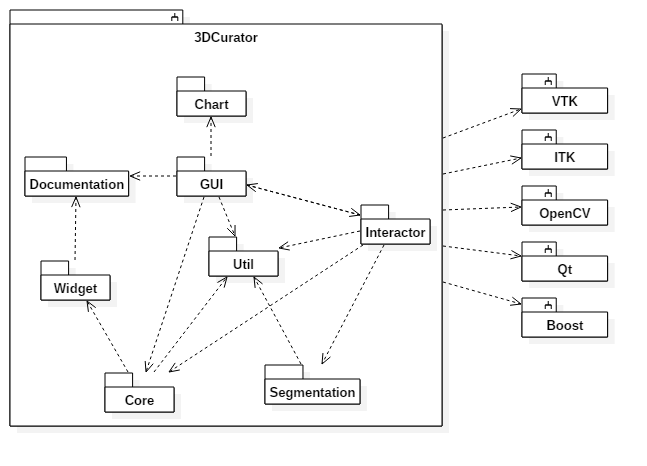
\includegraphics[width=12cm]{imagenes/diseno/package}
	\caption{Diagrama de paquetes de 3DCurator}
	\label{fig:diseno/package}
\end{figure}

\section{Diagramas de clases}

Se presentan las distintas clases de los distintos módulos que contiene 3Dcurator.

Estos diagramas se encuentran disponibles en la rama de diseño del repositorio del proyecto: \url{https://github.com/fblupi/3DCurator/tree/design} por si es necesario verlos a mayor tamaño.

\subsection{\textit{Chart}}

Este módulo contiene las clases auxiliares para controlar las gráficas utilizadas para visualizar y editar la función de transferencia:

\begin{figure}[H]
	\centering
	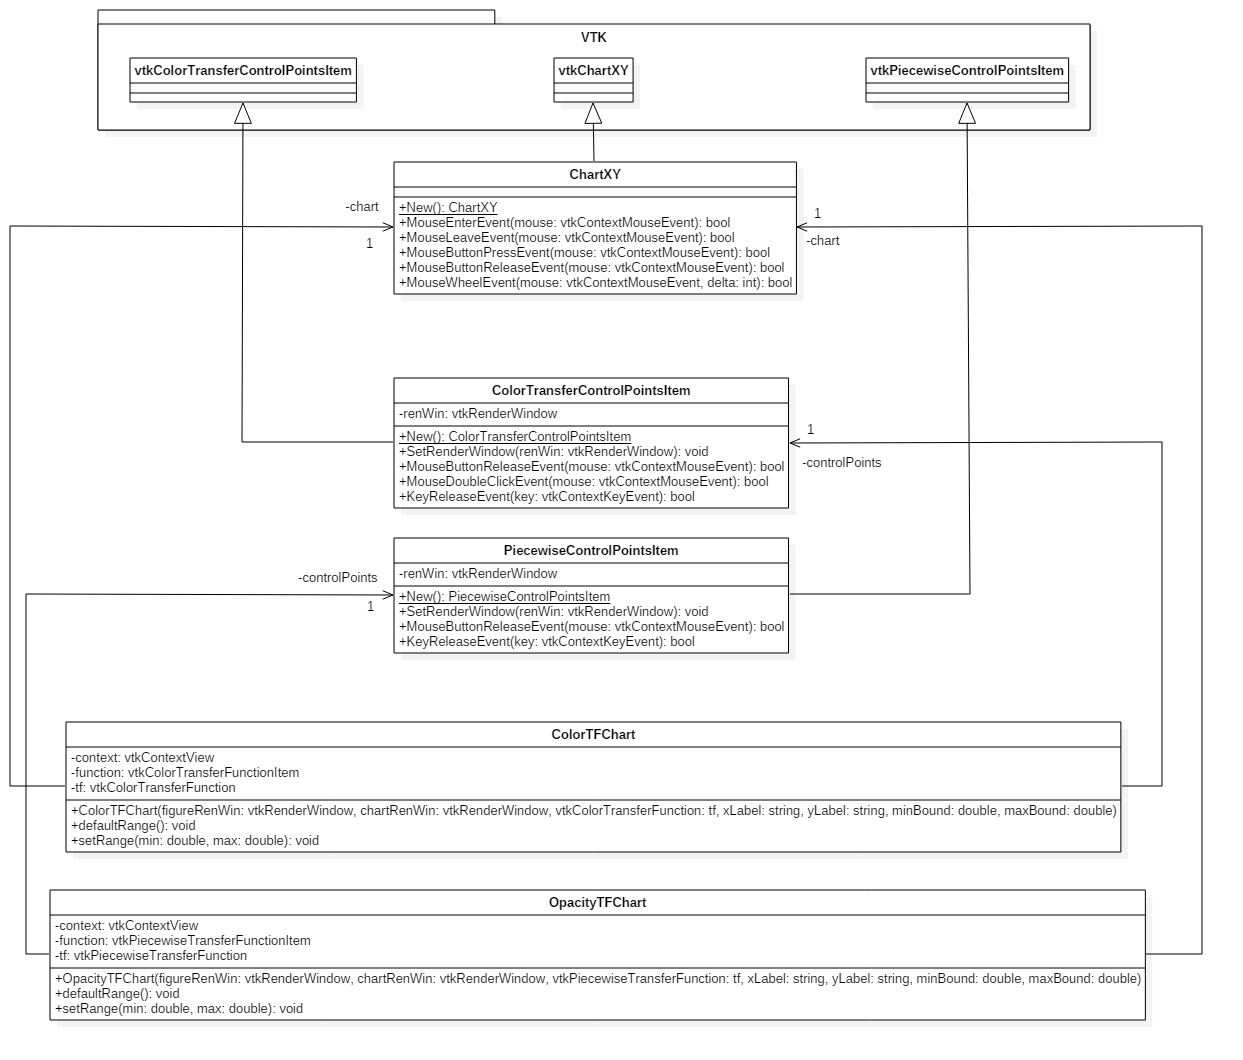
\includegraphics[width=12cm]{imagenes/diseno/chart}
	\caption{Diagrama de clases del paquete \textit{Chart}}
	\label{fig:diseno/chart}
\end{figure}

\subsection{\textit{Core}}

Este es el módulo principal de 3DCurator. Contiene las clases que gestionan los datos del volumen (\textit{Sculpture}), la función de transferencia (\textit{Transfer Function}) y plano de corte (\textit{SlicePlane}):

\begin{figure}[H]
	\centering
	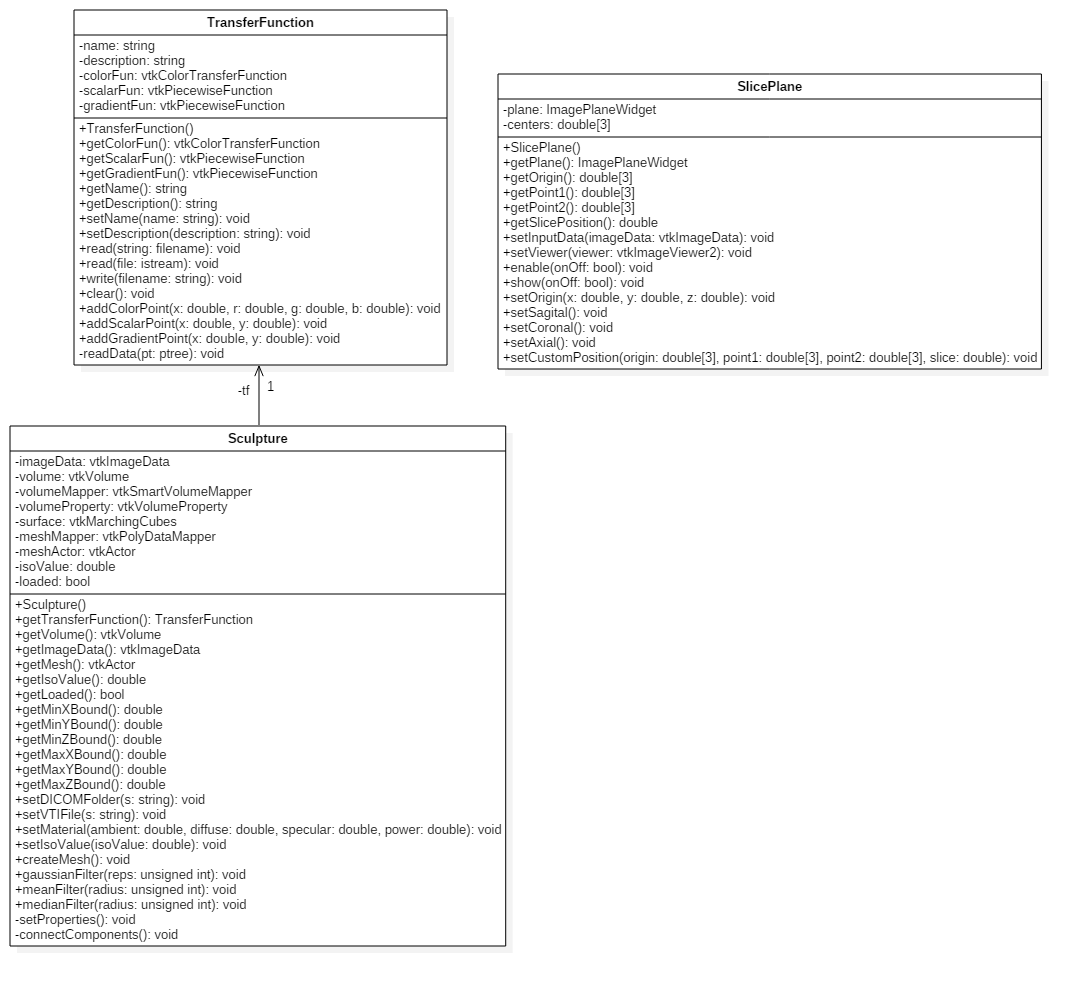
\includegraphics[width=12cm]{imagenes/diseno/core}
	\caption{Diagrama de clases del paquete \textit{Core}}
	\label{fig:diseno/core}
\end{figure}

\subsection{\textit{Documentation}}

En este módulo se encuentra la clase que almacena los distintos elementos utilizados para la documentación:

\begin{figure}[H]
	\centering
	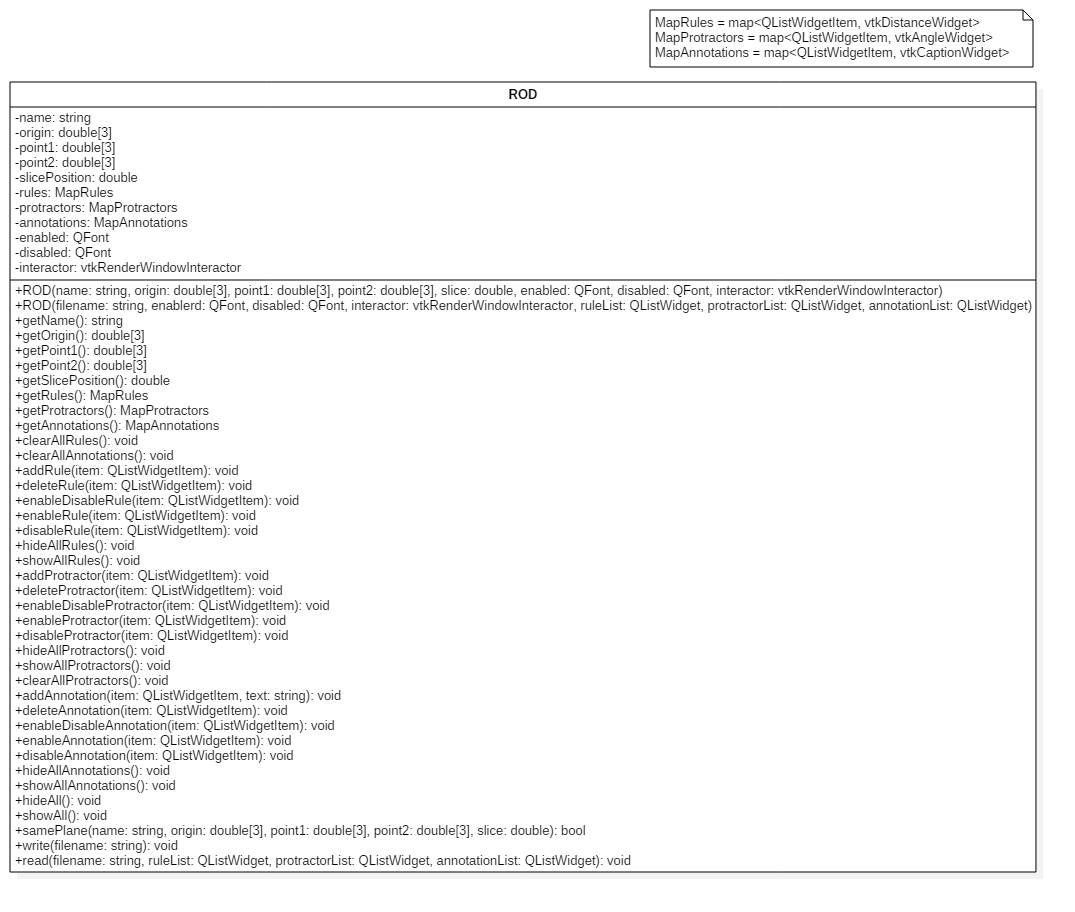
\includegraphics[width=12cm]{imagenes/diseno/documentation}
	\caption{Diagrama de clases del paquete \textit{Documentation}}
	\label{fig:diseno/documentation}
\end{figure}

\subsection{\textit{GUI}}

Este módulo contiene las distintas clases que gestionan las ventanas de la GUI:

\begin{figure}[H]
	\centering
	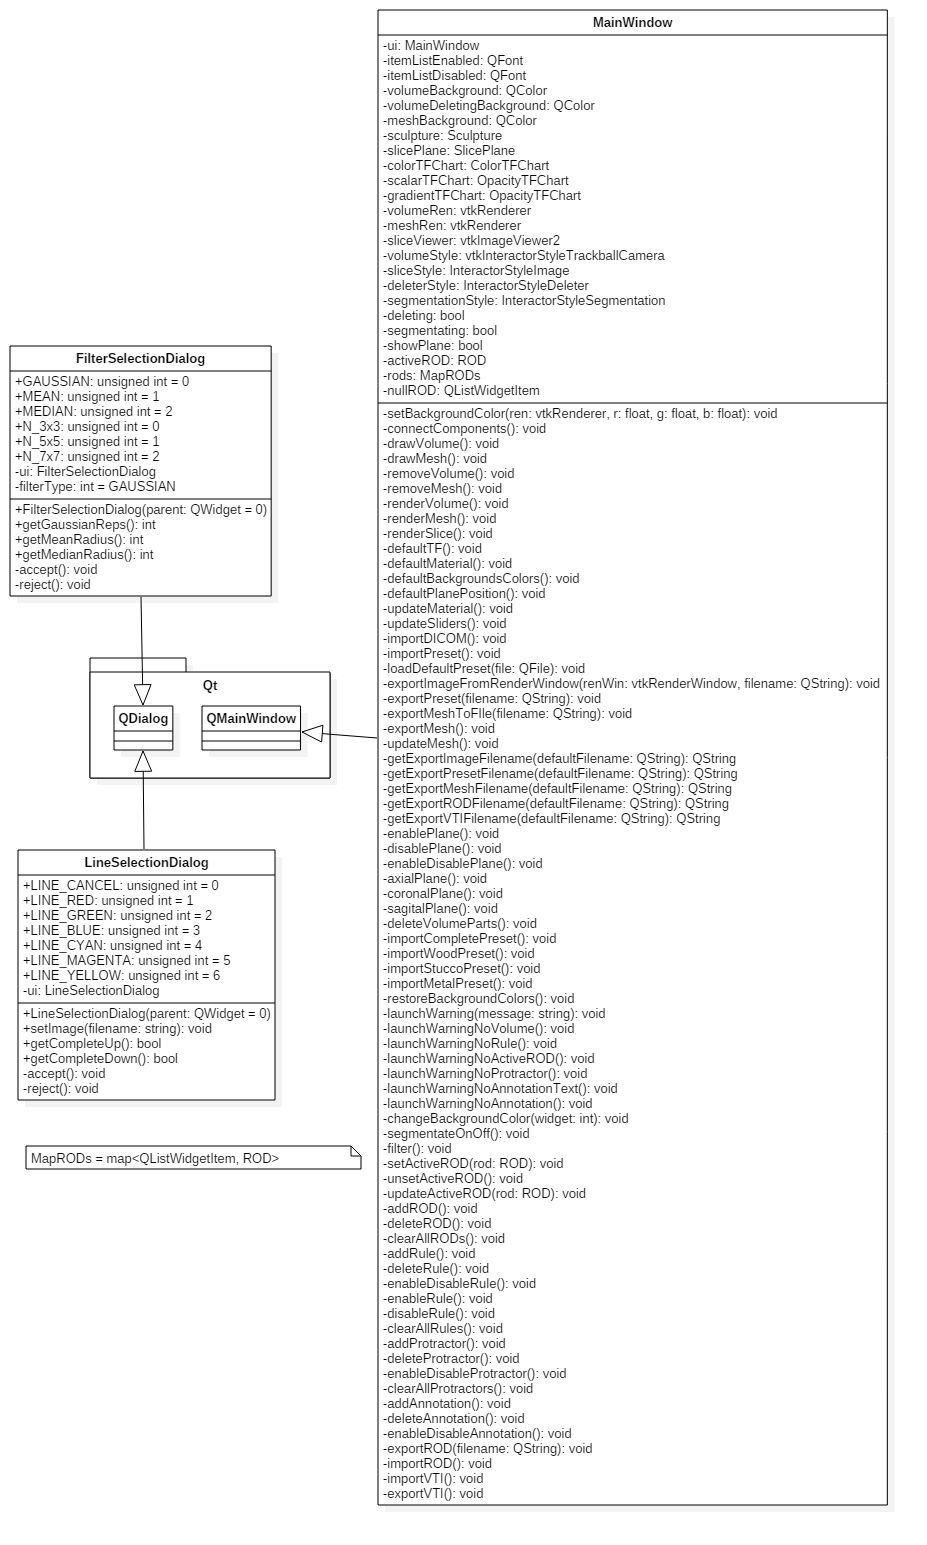
\includegraphics[width=12cm]{imagenes/diseno/gui}
	\caption{Diagrama de clases del paquete \textit{GUI}}
	\label{fig:diseno/gui}
\end{figure}

\subsection{\textit{Interactor}}

Este módulo contiene los distintos interactuadores con las ventanas de visualización: 

\begin{figure}[H]
	\centering
	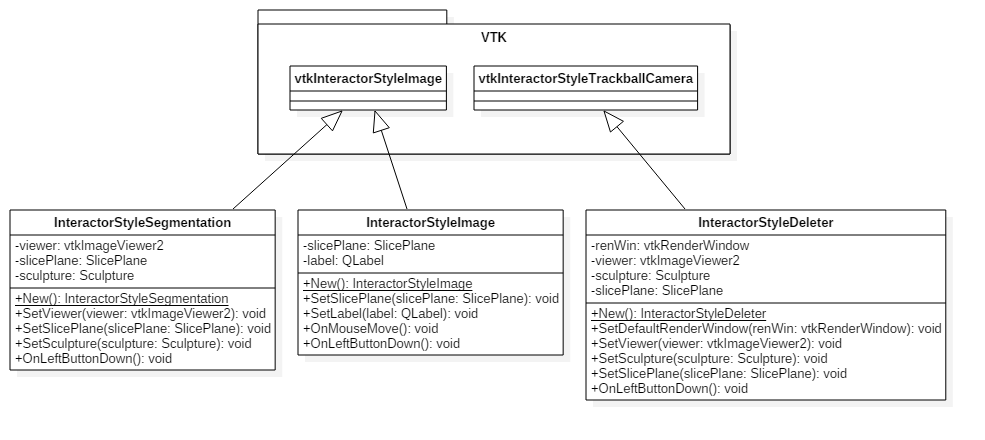
\includegraphics[width=12cm]{imagenes/diseno/interactor}
	\caption{Diagrama de clases del paquete \textit{Interactor}}
	\label{fig:diseno/interactor}
\end{figure}

\subsection{\textit{Segmentation}}

En este módulo se encuentran las clases utilizadas para realizar segmentaciones en el volumen:

\begin{figure}[H]
	\centering
	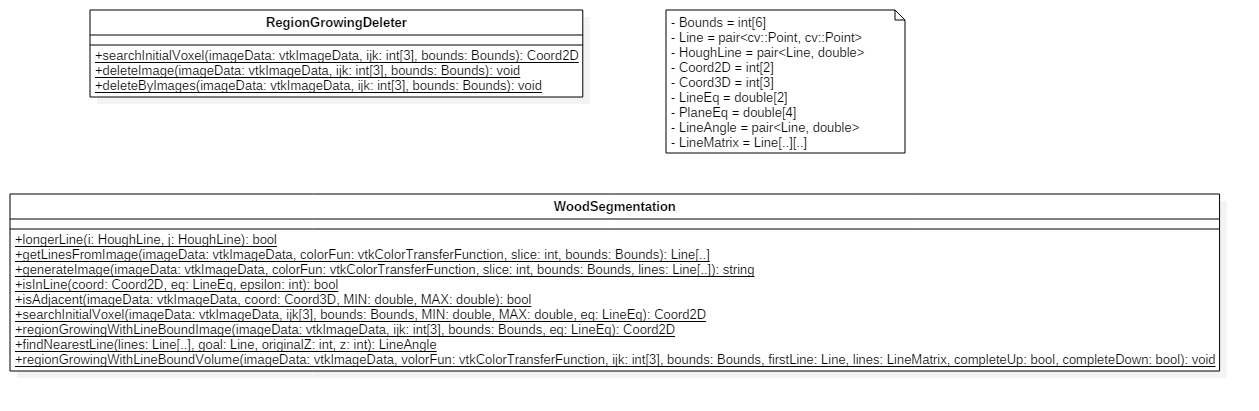
\includegraphics[width=12cm]{imagenes/diseno/segmentation}
	\caption{Diagrama de clases del paquete \textit{Segmentation}}
	\label{fig:diseno/segmentation}
\end{figure}

\subsection{\textit{Util}}

Este módulo contiene funciones utilizadas frecuentemente por distintos módulos del programa:

\begin{figure}[H]
	\centering
	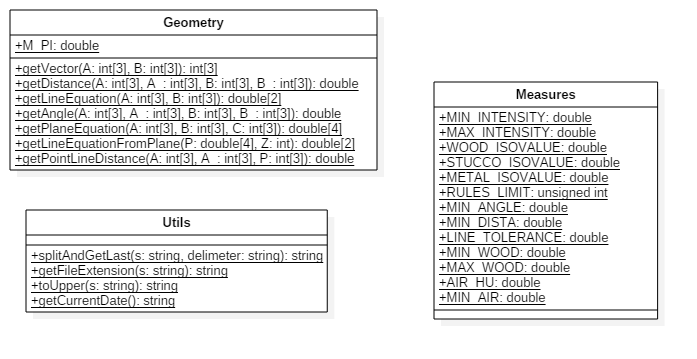
\includegraphics[width=12cm]{imagenes/diseno/util}
	\caption{Diagrama de clases del paquete \textit{Util}}
	\label{fig:diseno/util}
\end{figure}

\subsection{\textit{Widget}}

Este módulo contiene el \textit{widget} personalizado de VTK que se utiliza:

\begin{figure}[H]
	\centering
	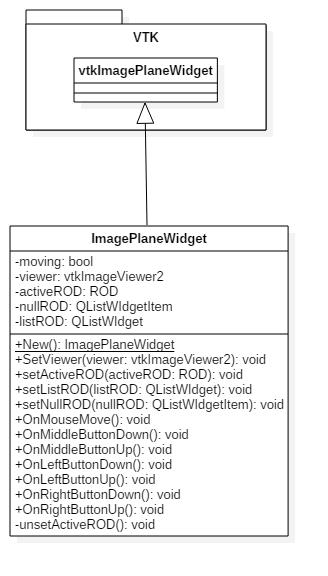
\includegraphics[width=5cm]{imagenes/diseno/widget}
	\caption{Diagrama de clases del paquete \textit{Widget}}
	\label{fig:diseno/widget}
\end{figure}